% Main chapter title
\chapter{Hauptkomponentenanalyse}

% Chapter label
\label{pca}

To Do: Kovarianzmatrix / Stichprobenkovarianzmatrix einheitlich!

Die Hauptkomponentenanalyse ist ein weitverbreitetes multivariates statistisches Verfahren zur Dimensionsreduktion. Multivariate Verfahren zielen darauf ab, die in einem Datensatz enthaltene Zahl der Variablen zu verringern, ohne die darin enthaltene Information (zu verlieren) / (wesentlich zu reduzieren). Dadurch können umfangreiche Datensätze strukturiert, veranschaulicht und vereinfacht werden. Somit ist das Verfahren Teil der explorativen Statistik, welche Datensätze hinsichtlich ihrer Zusammenhänge analysiert. Die sich ergebende Struktur kann für weitere Analysezwecke ausgenutzt werden.

Aus diesem Grund hat die Hauptkomponentenanalyse in vielen Bereichen erfolgreich Anwendung gefunden. Darunter fällt die Erkennung handgeschriebener Zahlen, welche zum Beispiel zur automatischen Sortierung von Briefen nach Postleitzahl genutzt wird \cite{hastie_elements}. An diesem Beispiel lässt es sich besonders gut verdeutlichen, was es heißt Zusammenhänge zu analysieren und Strukturen auf den Daten zu finden. Man erhofft, dass nach Anwendung einer Dimensionsreduktion wie PCA auf den Datensatz 10 verschiedene Gruppierungen zu erkennen sind, die für die Ziffern 0 bis 9 stehen (siehe dazu Bild?). Optimalerweise gehören alle Datenpunkte im demselbem Cluster zur selben Ziffer. Außerdem korrespondieren nahe beieinanderliegende Cluster mit Ziffern, die ähnlich aussehen. Weitere Anwendungen findet das Verfahren in der Bildverarbeitung. Hier kann es zum Beispiel zur Rauschunterdrückung \cite{babu} oder zur Gesichtserkennung \cite{jiang} genutzt werden. Um Bilder für solch ein Verfahren nutzbar zu machen, werden einzelne Pixel oder patches, also lokale Gruppierungen von Pixeln, eines Bildes als Variable interpretiert.

Das dahinterstehende mathematische Problem kann auf verschiedene Weisen beschrieben werden. Zunächst wollen wir die Hauptkomponentenanalyse so konstruieren, dass die Idee des minimalen Informationsverlust im Vordergrund steht. Anschließend werden wir das Problem auf eine Singulärwertzerlegung zurückführen, die auch zur effizienten Implementierung genutzt wird. Des Weiteren werden wir die Hauptkomponentenanalyse als Regressionsproblem betrachten und die geometrische Interpretation weiter verdeutlichen. Zu Schluss werden wir einige theoretische Aussagen angeben, die für die folgenden Kapitel relevant sind.

\section{Konstruktion}

Gegeben sei ein Datensatz mit $n$ samples und $p$ Variablen. Die zentrale Idee der Hauptkomponentenanalyse besteht darin, die $p$ bestehenden Variablen in $r$ neue, unkorrelierte Variablen zu überführen. Um eine Reduktion der Dimension, also $r < p$ zu erreichen, müssen die bestehenden Variablen \textit{zusammengefasst} werden. Idealerweise sollte bei diesem Prozess möglichst wenig Information verloren gehen. Als Maß für den Informationsgehalt der Daten wird hierbei die Varianz verwendet. Das heißt, je größer die Varianz einer Variable, desto mehr Information birgt sie und desto \textit{wichtiger} ist sie. Denn eine Variable, die für alle Beobachtungen ähnliche Werte aufweist, ist nicht von Nutzen bei der Unterscheidung verschiedener samples. PCA sucht also nach Eigenschaften, die hohe Varianz zeigen. Hierbei wählt das Verfahren aber nicht einfach nur bestimmte Eigenschaften mit hoher Varianz aus, sondern konstruiert neue Variablen, die die bestehenden zusammenfassen.

Abbildung Höhe Gewicht mit Eigenvektoren und gedrehtes Bild

Um dieses Prinzip zu veranschaulichen, wenden wir uns nun einem simplem Beispiel zu. Gegeben seien die Größe [cm] und das Gewicht [kg] zu 1000 Personen (Daten sind simuliert, keine real-world-data) (siehe dazu Abbildung). In diesem Fall ist also $n = 1000$ und $p = 2$. Bei Betrachtung der Abbildung fällt schnell auf, dass die beiden Variablen positiv korreliert sind, d.h. prinzipiell erkennt man folgende Tendenz: Je größer eine Person, desto schwerer ist sie. 

Konkret suchen wir also sukzessive nach einer Linearkombination der bestehenden Variablen. Diese Linearkombination sei so gewählt, dass der zugehörige Vektor in die Richtung größter Varianz in unserem Datensatz zeigt. Die so entstehenden Vektoren werden Hauptachsen bzw. Hauptrichtungen genannt. Nach der Berechnung der Hauptachsen wollen wir unsere Beobachtungen bezüglich der neuen Variablen darstellen. Dazu projizieren wir die einzelnen Beobachtungen auf die neuen Variablen. Die Werte gemäß der neuen Variablen werden Hauptkomponenten genannt. 

DIESE BEIDEN ABSÄTZE GUT ZUSAMMENFASSEN. Orthogonalität mit rein bringen, nach Wichtigkeit sortiert und sukzessive.  Anordnung nach absteigender Varianz bzw. Information.

Konkret konstruieren wir Variablen, die sich aus Linerakombinationen der Alten zusammensetzen. Dabei sollen die neuen Variablen der Wichtigkeit nach sortiert sein. In anderen Worten enthält die erste Variable die meiste Information bzw. die größte Varianz, dann die zweite, usw.

Die eigentliche Dimensionsreduktion findet dann durch Selektion statt. Je nach Komplexität des Modells, welches man erreichen möchte, können so mehr oder weniger Hauptkomponenten ausgewählt werden. Es kommt also auf den Anwendungsfall an, wie viele Hauptkomponenten auszuwählen sind. Wir werden uns mit diesem Thema aber weiter in CITE beschäftigen.
Insgesamt haben wir somit eine kleinere, neue Zusammenstellung von Variablen konstruiert, die aber trotzdem den Großteil an Information beinhaltet.

Bevor wir die Hauptkomponentenanalyse auf den Datensatz anwenden können, gibt es aber noch einen wichtigen Bearbeitungsschritt zu beachten. Wenn eine Variable weniger variiert als eine Andere aufgrund der verwendeten Einheit oder Skala (meter oder kilo) kann dies zu ungewollten Ergebnissen führen. Ohne eine Vorbehandlung der Daten hat so im obigen Beispiel eine Änderung von 1m die gleiche Bedeutung wie eine Änderung von 1kg. (Satz schöner formulieren) Allerdings sind zwei Menschen, deren Größe 1m variiert, sehr verschieden, während zwei Menschen, die eine Differenz von 1kg haben, sehr ähnlich sind. Daher werden die Daten häufig einem sog. preprocessing unterzogen. Ein zu diesem Zweck oft verwendetes Verfahren ist die Standardisierung (auch z-Transformation genannt). In diesem Schritt werden die Variablen so transfomiert, dass sie \textit{vergleichbarer} werden. Seien dazu $X_i$ die Zufallsvariablen mit Erwartungswert $E[X_i] = \mu$ und Varianz $Var[X_i] = \sigma^2$. So erhält man die zugehörigen standardisierten Zufallsvariablen $Z_i$ durch Zentrierung und anschließender Division durch die Standardabweichung $Z = \frac{X-\mu}{\sigma}$. Somit gilt dann:
\begin{itemize}
\item $E[Z_i] = 0$ für alle $1 \leq i \leq p$
\item $Var[Z_i] = 1$ für alle $1 \leq i \leq p$
\end{itemize}

Mathematisch gesehen wendet man das Verfahren also nicht auf die Kovarianzmatrix, sondern auf die Korrelationsmatrix an.

\subsection{Problemformulierung als Varianzmaximierung}

Wir wollen nun die Intuition des minimalen Informationsverlust mathematisch beschreiben. Gegeben sei dazu eine Matrix $\mat{X} \in \mathbb{R}^{n\times p}$, wobei $n$ die Anzahl der Samples bzw. Beobachtungen und $p$ die Anzahl der Variablen ist. Wir nehmen im Folgenden ohne Beschränkung der Allgemeinheit an, dass die Variablen zuvor zentriert wurden. Aufgabe der Hauptkomponentenanalyse ist es nun sukzessive Richtungen größter Varianz zu finden. Die erste Hauptkomponente ist definiert durch $Z_1 = \sum_{j=1}^p v_{1j}X_j = \mat{X}v$ wobei die Hauptachse $v_1 = (v_{11}, \ldots, v_{1p})^T$ so gewählt wird, dass die Varianz von $Z_1$ maximiert wird, d.h.
$$v_1 = \argmax_{\norm{v}_2 = 1} \text{Var}[\mat{X}v] = \argmax_{\norm{v}_2 = 1} v^T \mat{K}_{xx} v$$
mit $\mat{K_{xx}} = \frac{\mat{X}^T\mat{X}}{n-1}$ als Stichprobenkovarianzmatrix. Die restlichen Hauptachsen können nun sukzessive definiert werden.
$$v_{k+1} = \argmax_{\norm{v} = 1} v^T \mat{K}_{xx} v$$ 
$$v_{k+1}^Tv_l = 0 \quad \forall 1 \leq l \leq k$$
Man sucht also unter den Richtungen, die orthogonal zu allen bisherigen Hauptachsen sind, diejenige, die die Varianz maximiert. Wie oben beschrieben erhält man dann die Hauptkomponenten, also die Darstellung der Daten bezüglich der neu gefundenen Variablen, durch Projektion der Daten $Z_i = \mat{X}v_i$.
\cite{zou_overview}
CITE JOLLIFE

Wie wir bereits in THEOREM gesehen haben, entsprechen die Eigenvektoren der Kovarianzmatrix genau den Richtungen maximaler Varianz. Daher können wir anstatt sukzessiver Berechnung einzelner Hauptachsen die Kovarianzmatrix $\mat{K}_{xx}$ direkt diagonalisieren. Dies ist möglich, da $\mat{K}_{xx}$ symmetrisch ist. Die Diagonalisierung ergibt
$$\mat{K}_{xx} = \mat V \mat L \mat{V}^T$$
wobei $\mat V$ die Matrix der Eigenvektoren ist, d.h. jede Spalte entspricht einem Eigenvektor von $\mat{K}_{xx}$ und $\mat{L}$ eine Diagonalmatrix mit Eigenwerten $\lambda_i$ ist. Somit können die Hauptachsen direkt aus $\mat V$ abgelesen werden. Die Projektion der Daten auf die Hauptachsen wird dann wie zuvor durch Multiplikation der Beobachtungen mit den Eigenvektoren erreicht. 
$$\mat Z = \mat X \mat V$$
Die i-te Spalte in $\mat{Z}$ entspricht also der i-ten Hauptkomponente und die einzelnen Beobachtungen bezüglich der neuen Variablen stimmen mit den Zeilen von $\mat{Z}$ überein.


\subsection{Formulierung als Singulärwertzerlegung}
Es gibt einen engen Zusammenhang zwischen der Diagonalisierung der Kovarianzmatrix $\mat{K}_{xx} = \mat X^T \mat X$ und der Singulärwertzerlegung von $\mat X$. Diese Beziehung können wir nutzen, um das Problem neu zu formulieren. Eine Singulärwertzerlegung der Matrix $\mat X$ ergibt
$$ \mat{X} = \mat{U}\mat{D}\mat{V}^T $$
wobei $\mat{D}$ eine Diagonalmatrix mit Singulärwerten $d_1,\ldots,d_p$, $\mat{U}$ eine orthogonale $n \times p$ und $\mat{V}$ eine orthogonale $p \times p$ Matrix ist. Nun sieht man aufgrund der Orthogonalität von $\mat U$, dass
$$\mat{K}_{xx} = \mat X^T \mat X = \mat{V}\mat{D}\mat{U}^T \mat{U}\mat{D}\mat{V}^T = \mat V \mat{D}^2 \mat V^T$$
Wegen der Eindeutigkeit der Diagonalisierung(stimmt das?) ist $\mat V$ nun wie zuvor die Matrix der Eigenvektoren und somit der Hauptachsen. Ebenso stehen die Singulärwerte durch $\lambda_i = \frac{d_i^2}{n-1}$ in Beziehung mit den Eigenwerten der Kovarianzmatrix. Die Hauptkomponenten kann man somit auch durch $\mat X \mat V = \mat U \mat D$ erhalten.

Computing PCA using Eigen value decomposition of the sample covariance matrix:
We first have to compute the covariance matrix, which is $O(p^2n)$ and then compute its eigenvalue decomposition which is $O(p^3)$ giving a total cost of $O(p^2n+p^3)$ (https://arxiv.org/pdf/1503.05214.pdf)

Computing PCA using SVD of the data matrix:
Svd has a computational cost of $O(p^2n)$

Numerical Stability? Which method is preferrable in the $n << p$ case?


\subsection{Formulierung als beste Rang k Rekonstruktion}
Further multiplying the first k PCs by the corresponding principal axes $\mat V^T k$ yields $\mat X_k = \mat U_k \mat S_k \mat{V}_k^T$ matrix that has the original $n \times p$ size but is of lower rank (of rank k). This matrix $\mat X_k$ provides a reconstruction of the original data from the first k PCs. It has the lowest possible reconstruction error


\subsection{Formulierung als Regressionsproblem}

\begin{figure}
\centering
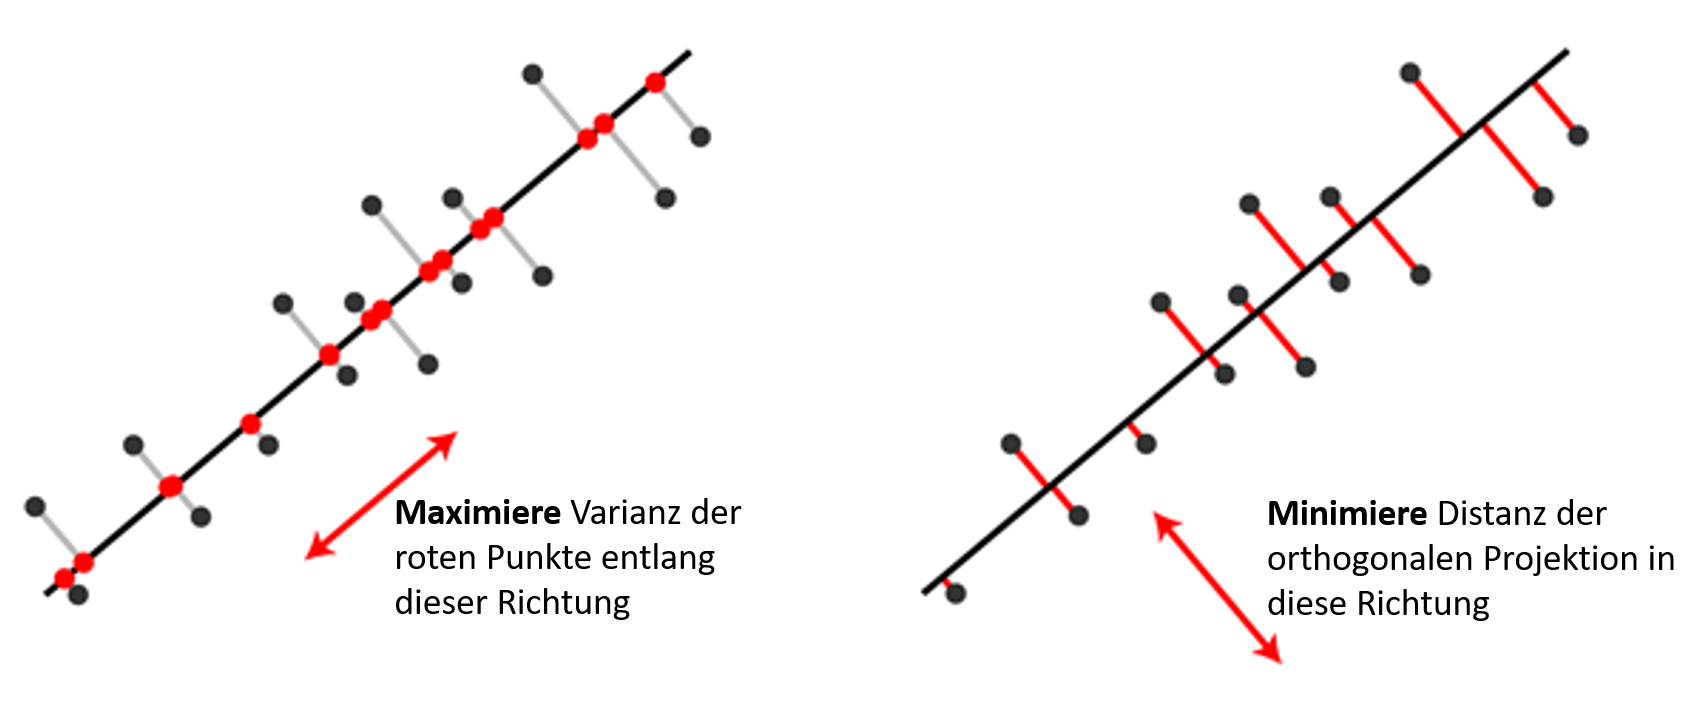
\includegraphics[width = 0.8\textwidth]{figures/pca_projection_explanation_german.png}
\caption{Die Abbildung zeigt die Äquivalenz von Maximierung der Varianz und Minimierung der Distanz der orthogonalen Projektion}
\label{pca_projection_explanation}
\end{figure}

Wir widmen uns nun einer letzten Formulierung der Hauptkomponentenanalyse, die eine geometrische Interpretation ermöglicht. Hierbei versucht man einen $k$-dimensionalen $(k < n)$ Unterraum zu finden, der die Daten bestmöglich im Sinne der kleinsten Quadrate approximiert. Wir werden diese Problemstellung nun mathematisch formulieren.

Sei dazu $x_i$ die i-te Beobachtung, also die i-te Zeile von $\mat X$ und $\mat V_k = [V_1 \vert \cdots \vert V_k]$ eine $p \times k$ orthonormale Matrix. Nun projizieren wir jede Beobachtung orthogonal auf den durch $V_1, \ldots V_k$ aufgespannten Unterraum. Die orthogonale Projektion wird wie in REF beschrieben durch Multiplikation mit dem Operator $\mat V_k \mat V_k^T$ erreicht. Die auf den linearen Unterraum projizierten Daten ergeben sich also durch $\mat V_k \mat V_k^T x_i$. Um die Daten bestmöglich in diesem niedrigdimensionalen Raum darzustellen minimiert man nun die Distanz zwischen jeder Beobachtung und seiner Projektion. Ein Weg, um die beste Projektion zu definieren is $l_2$ Approximation erhält man folgendes Problem \cite{zou_sparsepca}: (Hier auch noch schreiben warum man den zweiten Term braucht, Eindeutigkeit von PCA)

$$\hat{\mat{V}_k} = \argmin_{\mat{V}_k} \sum_{i=1}^{n} \norm{x_i - \mat{V}_k \mat{V}_k^Tx_i}^2 + \lambda \sum_{j=1}^{k}\norm{\beta_j}^2$$
$$\mat{V}_k^T\mat{V}_k = I_{k \times k}$$

Man kann zeigen, dass die Lösung des Problems $\mat V_k$ genau den ersten $k$ Hauptachsen entsprechen. Wir haben dies in \ref{theo_results} festgehalten.  \cite{vidal} Zum besseren Verständnis hilft \ref{pca_projection_explanation}, welches die Äquivalenz von Maximierung der Varianz und Minimierung der orthogonalen Projektion verdeutlichen soll. Jeder Datenpunkt ist hier in 2 Dimensionen dargestellt. Versucht man nun die Daten bestmöglich auf einen 1-dimensionalen Unterraum, also eine Linie, orthogonal zu projizieren erhält man denselben Vektor, den man bei der Maximierung der Varianz zuvor auch erhalten hat. 

Aus dieser Interpretation leitet sich auch der Name des linearen Dimensionreduktionsverfahren ab, denn die Daten werden auf den niedrigdimensionaleren Raum linear transformiert. Ausgehend von dieser Formulierung als Regressionsproblem werden wir im nächsten Kapitel die Variante der dünnbesetzten Hauptkomponentenanalyse beschreiben.


\section{Selektion der Hauptkomponenten}
Wie viele Hauptkomponenten sollen wir auswählen?

Abbildung Scree Plot

Optimal singular threshold \cite{gavish}

\section{Grenzen der Anwendbarkeit} \label{theo_results}

Obwohl die Hauptkomponentenanalysen in vielen Situationen helfen kann, Datensätze zu veranschaulichen und zu strukturieren, gibt es keine Garantie für sinnvolle Ergebnisse. Im Folgendem werden wir Szenarien beschreiben, bei denen unerwünschte Effekte bei der Verwendung dieses Verfahrens auftreten. Daher gilt es den Datensatz vorest hinsichtlich folgender Gesichtspunkte zu untersuchen: 

\begin{itemize}
\item Lineare Beziehung zwischen Variablen
\item Korrelation der Variablen
\item Vollständigkeit des Datensatzes
\item Ausreißer in den Daten
\item Anzahl an Beobachtungen in Relation zu Anzahl an Variablen
\end{itemize}

Wie in REF beschrieben versuchen wir Daten in einen niedrigdimensionaleren linearen oder affinen Unterraum zu transformieren. Es kann aber durchaus vorkommen, dass es keine lineare Beziehung zwischen den Variablen gibt. Nichtlineare Strukturen können von PCA nicht erfasst werden und gehen somit verloren. \cite{vidal} Vidal et al. zeigen diese Grenze konkret am Beispiel von Porträt-Fotos auf. Seit der Entstehung von PCA gab es aber zahlreiche nicht-lineare Erweiterungen. So nutzt zum Beispiel Kernel PCA den \textit{Kernel Trick} aus, bei welchem man die Daten zuerst durch eine nichtlineare Transformation in ein höherdimensionalen Raum einbettet von dem man sich erhofft, dass die Daten in diesem linear verteilt. Erst anschließend wird dann die eigentliche Reduktion durchgeführt. Hierbei muss man die Daten aber nicht im höherdimensionalen Raum auswerten. CITE. Andere Erweiterungen, die allgemein unter \textit{manifold learning} zusammengefasst werden können, basieren auf der Idee, dass die Dimension des Datensatz nur künstlich hoch ist. Man versucht die lokale Geometrie der Mannigfaltigkeit (Begriff erklären?) zu approximieren und damit direkt eine niedrigdimensionale Einbettung zu erhalten. Hierunter fallen zum Beispiel die multidimensionale Skalierung oder ISOMAP.

Damit der Datensatz für eine Dimensionsreduktion per PCA geeignet ist, müssen die verschiedenen Variablen einen gewissen Grad an Korrelation aufweisen. Im extremen Fall der Unabhängigkeit der Variablen bewirkt eine Hauptachsentransformation nichts. Reduziert man dann die Anzahl der Hauptkomponenten verliert man mit jeder Variable einen Großteil der Information.

Ein weiterer Gesichtspunkt ist die Vollständigkeit eines Datensatzes. Finden wir fehlende oder korrupte Einträge in unserem Datensatz vor, kann die klassische Hauptkomponentenanalyse ... . Für dieser Art Probleme existieren entsprechende Ergänzungen von PCA wie zum Beispiel in cite und cite. Ausreißer in den Daten können die Resultate drastisch beeinflussen. Genaue Effekte überlegen und CITE. Aus diesem Grund sollten Ausreißer vor der Anwendung von PCA entfernt werden.

Außreiser in den Daten.

Anzahl der Variablen zu hoch.

Darüber hinaus gibt es noch eine Reihe Spezialfälle, bei denen Probleme auftreten können. So kann es zum Beispiel passieren, dass die relevanten Informationen in den Variablen mit niedriger Varianz versteckt sind. Da die Hauptkomponentenanalyse gerade diese Variablen vernachlässigt, wird sich unter Umständen nicht die erwünschte Struktur auf den Daten ergeben. Es bedarf anderer Methoden mit anderen Ansätzen, um eine Dimensionsreduktion zu ermöglichen. Oftmals weiß man aber im Vorhinein nicht, in welchen Variablen diese Unterscheidungsmöglichkeit versteckt ist.

Das wohl wichtigste/größte Hindernis im Zuge dieser Arbeit ist sicherlich die durch die Transformation entstehenden Interpretationsschwierigkeiten. Jede Hauptkomponente entsteht wie oben beschrieben durch eine Linearkombination der Ausgangsvariablen. Während die Ausgangsvariablen Bedeutungen wie Gewicht oder Größe hatten ist in vor allem in hochdimensionalen Fällen eine Interpretation der Hauptkomponenten nur schwer möglich (Rotation Techniques CITE). Dieser Interpretationsverlust ist Ausgangspunkt der Idee der dünnbesetzten Hauptkomponentenanalyse, genannt sparse PCA. Diesem Verfahren ist das folgende Kapitel gewidmet.


\section{Theoretische Aussagen}

\begin{thm}
PCA always gives unique solution.
\end{thm}

\begin{thm}[\cite{vidal}]
Sei $\mat X \in \mathbb{R}^n$ und $\mat A_{p,k} = [\alpha_1, \ldots \alpha_k] $   
\end{thm}

\begin{thm}
PCA inconsistent for n << p.
\end{thm}

